\documentclass[a4paper,11pt]{ctexart}
\usepackage{times}
\usepackage{setspace}
\usepackage{fancyhdr}
\usepackage{graphicx}
\usepackage{wrapfig}
\usepackage{array}  
\usepackage{fontspec,xunicode,xltxtra}
\usepackage{titlesec}
\usepackage{titletoc}
\usepackage[titletoc]{appendix}
\usepackage[top=30mm,bottom=30mm,left=20mm,right=20mm]{geometry}
\usepackage{cite}
\usepackage{listings}
\usepackage[table]{xcolor}
\usepackage{amsmath,bm}
\usepackage{amssymb}
\usepackage{easybmat}
\usepackage{color}
\usepackage{enumerate}

\usepackage{colortbl}


\usepackage{multicol} %表格宏包 
\usepackage{multirow} 
\usepackage{booktabs}  
\usepackage{threeparttable}
\usepackage{longtable}
\usepackage{rotating}
\usepackage{diagbox} 
\usepackage{ ntheorem} 

%tikz绘图
\usepackage{tikz}
\usepackage[T1]{fontenc}
\usepackage[utf8]{inputenc}
\usepackage{pgfplots}
\usepackage{grffile}
\pgfplotsset{compat=newest}
\usetikzlibrary{plotmarks}
\usetikzlibrary{arrows.meta}
\usepgfplotslibrary{patchplots}

\usepackage{subfigure}
\usepackage{float}
%设置页眉与页脚
\usepackage{fancyhdr}
\usepackage{pythonhighlight} %自定义python代码插入
\pagestyle{fancy}
\fancyhf{}
\chead{应用tensorflow实现简单的机器学习}
\cfoot{\thepage}
%\fancyfoot[LE,RO]{\thepage}
%\fancyhead[CE]{ 高等数值分析课程大作业 }
%\fancyhead[CO]{\section}
%\fancyhead[RO]{\thepage} %奇数页眉的右边
%\fancyhead[LE]{\thepage} %偶数页眉的左边
%\chead{\rightmark}

%\fancyhead[LO]{\rightmark}


%设置交叉引用的格式
%\usepackage[colorlinks,linkcolor=black,anchorcolor=blue,citecolor=green,pdfstartview=FitH]{hyperref}
\usepackage[CJKbookmarks=true,
bookmarksnumbered=true,
bookmarksopen=true,
colorlinks=true,
pdfborder=001,
citecolor=blue,
linkcolor=blue,
anchorcolor=green,
urlcolor=blue,
pdfstartview=FitH,
pdftitle={Python机器学习及大数据处理},
pdfauthor={LiAsNH3},
pdfsubject={应用tensorflow实现简单的机器学习},
pdfkeywords={Tensorflow,卷积神经网络,猫狗图集},
pdfcreator={XeTeX,XeCJK},
pdfproducer={XeTeX},% 这个好像没起作用? 
]{hyperref}
%算法描述宏包
\usepackage[ruled,algosection,vlined]{algorithm2e}
%\usepackage{algorithm2e}
\renewcommand{\algorithmcfname}{算法}%标题中文化

%\pagestyle{plain}
\setmainfont{Times New Roman}%设置全文英文字体为time new Roman,中文字体默认为宋体

%设置输入的代码的颜色
\definecolor{mygrey}{gray}{0.9}
\definecolor{grey}{rgb}{0.8,0.8,0.8}
\definecolor{darkgreen}{rgb}{0,0.3,0}
\definecolor{darkblue}{rgb}{0,0,0.3}
\def\lstbasicfont{\fontfamily{pcr}\selectfont\footnotesize}
\lstset{%
	 numbers=left,
	% numberstyle=\small,%
	showstringspaces=false,
	showspaces=false,%
	tabsize=4,%
	frame=lines,%
	basicstyle={\footnotesize\lstbasicfont},%
	keywordstyle=\color{blue}\bfseries,%
	identifierstyle=,%
	commentstyle=\color{darkgreen},%\itshape,%
	stringstyle=\color{black}%
}
\lstloadlanguages{C,C++,Java,Matlab,Mathematica}


%---------------------------------------------------------------------
%	章节标题设置
%---------------------------------------------------------------------
\titleformat{\section}{\centering\zihao{-3}\heiti}{\chinese{section}、}{0.1em}{}
\titlespacing{\section}{0pt}{*1}{*0.5}%设置标题与上下段落的间距
\titlespacing{\subsection}{0pt}{*0.5}{*0}%设置标题与上下段落的间距
\titlespacing{\subsubsection}{0pt}{*0}{*0}%设置标题与上下段落的间距
%---------------------------------------------------------------------
%	摘要标题设置
%---------------------------------------------------------------------
\renewcommand{\abstractname}{\zihao{-3} 说\quad 明}
\renewcommand{\contentsname}{\zihao{-3} 目\quad 录}

%---------------------------------------------------------------------
%	参考文献设置
%---------------------------------------------------------------------
\renewcommand{\refname}{\zihao{-3}{\hspace{\fill}参\hspace{0.5em}考\hspace{0.5em}文\hspace{0.5em}献\hspace{\fill}}}

%---------------------------------------------------------------------
%	引用文献设置为上标
%---------------------------------------------------------------------
\makeatletter
\def\@cite#1#2{\textsuperscript{[{#1\if@tempswa , #2\fi}]}}
\makeatother

%---------------------------------------------------------------------
%	目录页设置
%---------------------------------------------------------------------
\titlecontents{section}[0em]{\heiti\zihao{4}}{\thecontentslabel\ }{}{\hspace{.5em}\titlerule*[4pt]{$\cdot$}\contentspage}
\titlecontents{subsection}[2em]{\vspace{0.1\baselineskip}\songti\zihao{-4}}{\thecontentslabel\ }{}{\hspace{.5em}\titlerule*[4pt]{$\cdot$}\contentspage}
\titlecontents{subsubsection}[4em]{\vspace{0.1\baselineskip}\songti\zihao{-4}}{\thecontentslabel\ }{}{\hspace{.5em}\titlerule*[4pt]{$\cdot$}\contentspage}

%设置公式标号格式
\renewcommand{\theequation}{\arabic{section}.\arabic{subsection}.\arabic{equation}}
\renewcommand{\thetable}{\arabic{section}-\arabic{table}}
\renewcommand{\thefigure}{\arabic{section}-\arabic{figure}}
\makeatletter
\@addtoreset{equation}{subsection}
\@addtoreset{table}{section}
\@addtoreset{figure}{section}
\makeatother
%\numberwithin{equation}{section}

%定理环境`
\theoremstyle{break}
\newtheorem{suppose}{假设}[section]
\theoremstyle{plain}
\newtheorem{theorem}{定理}[section]

\setlength{\baselineskip}{20pt}
\begin{document}

\newcommand{\song}{\CJKfamily{song}}
\newcommand{\hei}{\CJKfamily{hei}}
\newcommand{\fang}{\CJKfamily{fang}}
\newcommand{\kai}{\CJKfamily{kai}}
\newcommand{\nwpulogo}{\CJKfamily{nwpulogo}}

%%%%%%%%%%%%%%%%%%%%%%%%%%%%%%%%%%%%%%%%%%%%%%%%%%%%%%%%%%%
% 重定义字号命令
%%%%%%%%%%%%%%%%%%%%%%%%%%%%%%%%%%%%%%%%%%%%%%%%%%%%%%%%%%%

\newcommand{\chuhao}{\fontsize{42pt}{63pt}\selectfont}    % 初号, 1.5倍行距
\newcommand{\yihao}{\fontsize{26pt}{36pt}\selectfont}    % 一号, 1.4倍行距
\newcommand{\erhao}{\fontsize{22pt}{28pt}\selectfont}    % 二号, 1.25倍行距
\newcommand{\xiaoer}{\fontsize{18pt}{18pt}\selectfont}    % 小二, 单倍行距
\newcommand{\sanhao}{\fontsize{16pt}{24pt}\selectfont}    % 三号, 1.5倍行距
\newcommand{\xiaosan}{\fontsize{15pt}{22pt}\selectfont}    % 小三, 1.5倍行距
\newcommand{\sihao}{\fontsize{14pt}{21pt}\selectfont}    % 四号, 1.5倍行距
\newcommand{\banxiaosi}{\fontsize{13pt}{16.25pt}\selectfont}    % 半小四, 1.25倍行距
\newcommand{\xiaosi}{\fontsize{12.5pt}{12.5pt}\selectfont}    % 小四, 1.2倍行距
\newcommand{\dawuhao}{\fontsize{11pt}{11pt}\selectfont}    % 大五号, 单倍行距
\newcommand{\wuhao}{\fontsize{10.5pt}{10.5pt}\selectfont}    % 五号, 单倍行距
\newcommand{\xiaowu}{\fontsize{9pt}{9pt}\selectfont}		% 小五号



%%%%%%%%%%%%%%%%%%%%%%%%%%%%%%%%%%%%%%%%%%%%%%%%%%%%%%%%%%%
% 重定义一些正文相关标题
%%%%%%%%%%%%%%%%%%%%%%%%%%%%%%%%%%%%%%%%%%%%%%%%%%%%%%%%%%%
\makeatletter
\newcommand\dlmu@underline[2][5cm]{\hskip1pt\underline{\hb@xt@ #1{\hss#2\hss}}\hskip3pt}
\let\coverunderline\dlmu@underline
\makeatother
%%%%%%%%%%%%%%%%%%%%%%%%%%%%%%%%%%%%%%%%%%%%%%%%%%%%%%%%
% 设置行距和段落间垂直距离
%%%%%%%%%%%%%%%%%%%%%%%%%%%%%%%%%%%%%%%%%%%%%%%%%%%%%%%%





\graphicspath{{result_figure/}}	
	
%---------------------------------------------------------------------------
%
%   封面设置
%
%---------------------------------------------------------------------------
\begin{titlepage}
	\voffset 2.0cm
	\begin{center}
		\begin{center}
			\begin{minipage}[c]{2.64cm}
				\centering
				\includegraphics[width=1.64 cm]{logo1.png}
			\end{minipage}
			\hskip 1.5 cm
			\begin{minipage}[c]{8cm}
				\includegraphics[scale=0.6]{logo2.png}
			\end{minipage}
		\end{center}
		\vskip 0.8cm
		\chuhao\song {\bfseries Python机器学习\\及大数据}
		\vskip 3cm
		{
			\sanhao\hei 题~~目 \hspace{0.2cm}\coverunderline[12.5cm]{应用tensorflow实现简单的机器学习}
		}
		\vskip 2cm
		{
			\sihao\song 学生姓名\coverunderline[7cm]{LiAsNH3}
			\vskip 0.7cm
			\sihao\song 学生学号\coverunderline[7cm]{xxxxxxxx}
			\vskip 0.7cm
			\sihao\song 学院名称\coverunderline[7cm]{xxxxxxxx}
			\vskip 0.7cm
			\sihao\song 专业名称\coverunderline[7cm]{xxxxxxxx}
			\vfill
		}
	\end{center}
\end{titlepage}


%--------------------------------------------------------------
%声明
%--------------------------------------------------------------
\thispagestyle{empty}
\begin{abstract}
\zihao{-4}
随着机器学习的发展,诞生了众多的机器学习(深度学习)框架,如TensorFlow、PyTorch、Caffe等,本文选择了社区较为丰富的TensorFlow架构来实现机器学习领域一些简单的算法。
\vspace{0.5em}\\
{\heiti 计算平台}\\
本文所有的算法均用Python实现,其版本为3.5.6;计算机性能如下:
\begin{itemize}
	\item 处理器:Intel(R)Core(TM)i7-7700 CPU @3.60GHZ
	\item 内存大小:8G
	\item 操作系统:Windows10家庭版
	\item GPU:计算能力3.5,GeForce GT 730
\end{itemize}
\vspace{0.5em}

\noindent{\heiti 数据集}\\
本文所使用的训练图像集来源于网上,共两类,猫有,狗有
测试图像集为百度图片里的,共采集了,其中猫,狗
\vspace{0.5em}\\

\noindent{\heiti 使用到的Python工具包}\\
下面列出用到的Python工具包以及他们的功能:
\begin{itemize}
	\item tensorflow-gpu:机器学习架构
	\item matplotlib:绘图相关
	\item numpy:数值计算相关(主要是矩阵相关的操作)
	\item PIL:图像处理相关
	\item random:产生随机数,返回类型为numpy中的数组
	\item requests:网络爬虫相关
	\item 以及上述的依赖包(具体见提供的Anaconda包列表文件TensorFlow-env.txt)
\end{itemize}
\end{abstract}
\newpage
\tableofcontents

\newpage
\section{小试牛刀 --- tensorflow的简单尝试}
\subsection{应用机器学习的方法实现数据拟合}
数据拟合是一种在数据处理中常用的方法,它能够反映数据的变化趋势,对于线性拟合的研究已经比较多了,有众多的实现方法;而对于非线性的拟合较为复杂,下面考虑一个二维区域上的非线性数据拟合,通过机器学习的方法来实现。
由于所考虑的问题为非线性的,因此需要考虑应用特殊激活函数来实现去线性化,在图中给出了几种常用的非线性激活函数的函数图像。
\begin{figure}[h]
	\centering
	\subfigure[ReLU函数$f(x)=max(x,0)$]{
		\includegraphics[width=0.3\linewidth]{relu_function.eps}
	}%
	\subfigure[sigmoind函数$f(x)=\frac{1}{1+e^{-x}}$]{
			\includegraphics[width=0.3\linewidth]{sigmoind_function.eps}
	}%
	\subfigure[$\tanh$函数$f(x)=\frac{1-e^{-2x}}{1+e^{-2x}}$]{
			\includegraphics[width=0.3\linewidth]{tanh_function.eps}
	}%
	\centering
	\caption{常用的神经网络非线性激活函数\label{fig:function}}
\end{figure}
从图\ref{fig:function}上可以看出,这些激活函数都不是一条直线,所以通过这些激活函数,每一个节点都不是线性变换,于是整个神经网络也不是线性的了。为简单起见,此处选取激活函数ReLU,构造了一个只有一层隐藏层的简单神经网络。
\subsubsection{数据点集}
通过产生随机数,在二维区域得到了一些带有噪声的数据点,如图\ref{fig:fit_data}所示。
\begin{figure}[h]
	\centering
	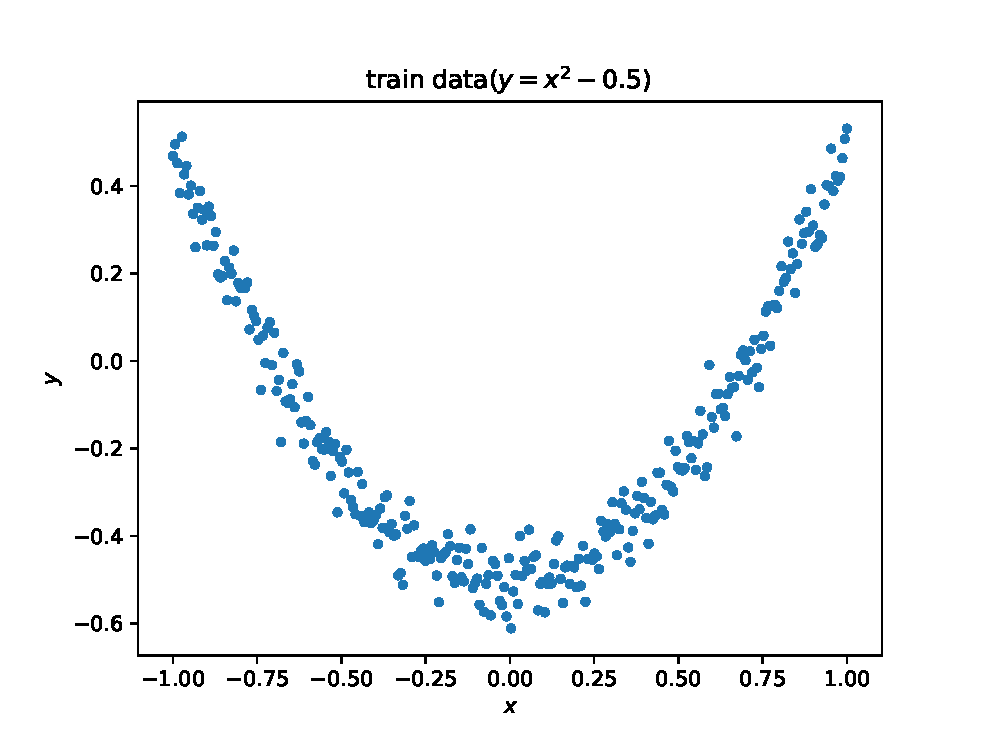
\includegraphics[scale=0.6]{fiting_trian.eps}
	\caption{需要拟合的二维数据\label{fig:fit_data}}
\end{figure}
事实上,这些数据是由$y=x^2-0.5+noise$得到的。接下来的任务就是通过机器学习得到这些数据点的最好近似。
\subsubsection{tensorflow实现}
下面给出tensorflow实现机器学习的步骤(根据具体的代码来说明):
\begin{itemize}
	\item 应用tensorflow实现数据拟合首先需要导入Python的工具包\footnote{代码见文件small\_try.py}
	\inputpython{C:/Users/lsa/Desktop/deep_learning/cats_and_dogs/small_try.py}{1}{6}
	\item 训练数据准备\\此处给定一个非线性函数,随机在图像上取点并加上一个噪声项,此处还通过matplotlib中scatter函数将其绘制出来,结果见图\ref{fig:fit_data}。
	\inputpython{C:/Users/lsa/Desktop/deep_learning/cats_and_dogs/small_try.py}{9}{20}
	\item 设置变量\\
	通过tensorflow的内置函数placeholder定义输入和输出信息,事实上tensorflow通过placeholder对数据进行了封装,为后续训练数据导入模型提供了方便。
	\inputpython{C:/Users/lsa/Desktop/deep_learning/cats_and_dogs/small_try.py}{23}{25}
	\item 创建损失函数和计算模型\\
	定义整个神经网络的各层设置,首先自定义了一个网络层函数
	\inputpython{C:/Users/lsa/Desktop/deep_learning/cats_and_dogs/small_try.py}{28}{49}
	接下来利用网络层函数定义输入层、隐藏层、输出层,并且隐藏层选用的激活函数为ReLU激活函数。
	\inputpython{C:/Users/lsa/Desktop/deep_learning/cats_and_dogs/small_try.py}{52}{55}
	损失函数是刻画当前预测值与真实答案之间的差距,在机器学习中一般通过反向传播算法来调整神经网络参数的取值使得差距缩小。下面通过预测值与真实值之间的平均欧式距离来定义的损失函数,定义了学习虑为0.1的以梯度下降法为优化方法反向传播。
	\inputpython{C:/Users/lsa/Desktop/deep_learning/cats_and_dogs/small_try.py}{57}{60}
	\item 将数据导入模型,创建会话,训练模型\\
	此处所考虑的问题较为简单,并且是空间二维的,所以通过matplotlib包中的绘图函数实现了模型在训练过程中预测值随着迭代进行的动态变化情况。
	\inputpython{C:/Users/lsa/Desktop/deep_learning/cats_and_dogs/small_try.py}{62}{93}
	\item 结果处理(可视化等)\\
	将迭代最终的预测结果、真实结果、训练数据绘制在一张图中,可视化训练结果。
	\inputpython{C:/Users/lsa/Desktop/deep_learning/cats_and_dogs/small_try.py}{95}{99}
\end{itemize}
\subsubsection{结果相关}
运行上述程序,得到训练的预测结果、真实函数形状、训练点三者的图示,见图\ref{fig:fit_result}。
\begin{figure}[h]
	\centering
	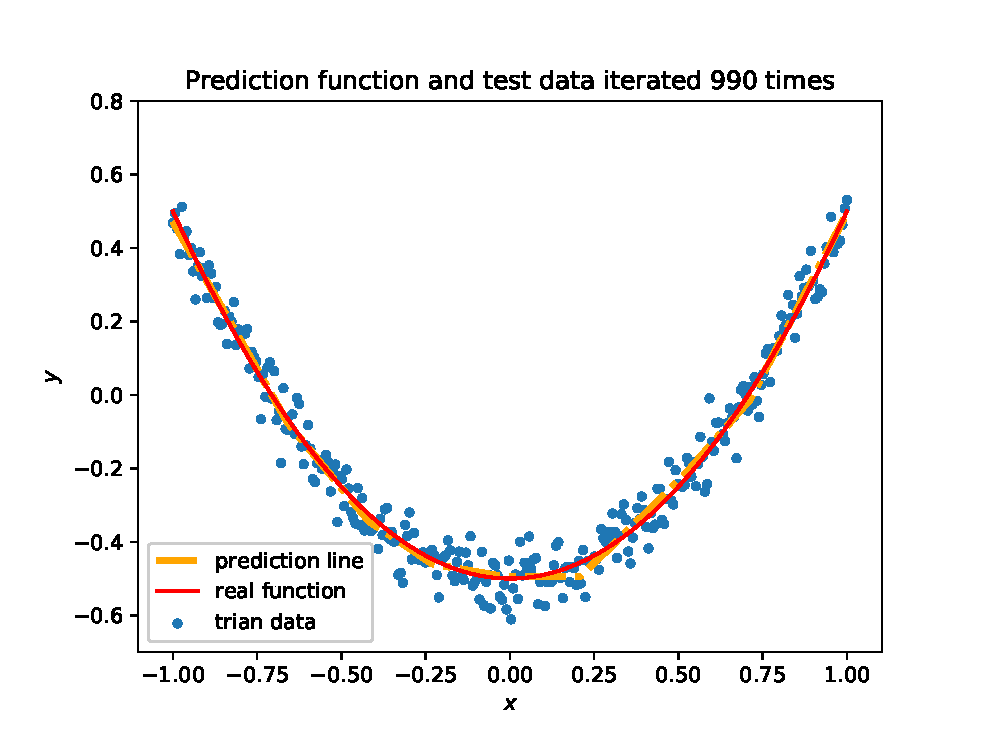
\includegraphics[scale=0.6]{fiting_result.eps}
	\caption{需要拟合的二维数据\label{fig:fit_result}}
\end{figure}
从图上来看,使用测试数据训练得到的结果可以很好近似原函形状。但实际上,机器学习方法很难显示的得到一个显示表达式,只能将其看做一个黑箱,输入一个数据,得到一个结果,数据与结果之间的这种抽象关系近似满足原函数。
\subsection{应用机器学习方法实现二维区域上的简单数据二分类}
下面来考虑机器学习中经典问题,对二区域上的点集进行分类,为简单起见这儿仅考虑对数据进行二分类。考虑单位正方形上的随机点,并且通过直线$x+y-1=0$将其分为两类,应用tensorflow编程实现。此处所考虑的神经网络有一层输入层,一层隐藏层,一层输出层,并且考虑了偏置项\footnote{代码实现见文件sample\_tensorflow.py}。
\subsubsection{tensorflow实现}
\begin{itemize}
	\item 导入必须的Python工具包tensorflow、matplotlib、numpy
	\inputpython{C:/Users/lsa/Desktop/deep_learning/cats_and_dogs/sample_tensorflow.py}{1}{7}
	\item 定义模型相关的参数权重、偏置项,以及输入、输出量
	\inputpython{C:/Users/lsa/Desktop/deep_learning/cats_and_dogs/sample_tensorflow.py}{10}{15}
	\item 定义前向传播过程及其损失函数
	\inputpython{C:/Users/lsa/Desktop/deep_learning/cats_and_dogs/sample_tensorflow.py}{18}{21}
	使用sigmoid函数将隐藏层输出转化为0到1之间的数值,转化后$y$代表预层是正样本的概率,$1-y$代表预层是负样本的概率。在上述代码中cross\_entropy定义了真实值与预测值之间的交叉熵,这是分类中常用的损失函数;为了保证结果的合理性,防止出现计算机无法表示的小数,将sigmoid函数转化的结果限制到$10^{-10}\textasciitilde 1$之间。train\_step定义了反向传播算法\footnote{tensorflow中目前常用的优化方法有三种:tf.train.GradientDescentOptimizer、tf.train.AdamOptimizer和tf.train.MomentumOptimizer}。
	\item 生成模拟训练数据集和测试数据集
	\inputpython{C:/Users/lsa/Desktop/deep_learning/cats_and_dogs/sample_tensorflow.py}{24}{34}
	\item 定义正确率计算
	\inputpython{C:/Users/lsa/Desktop/deep_learning/cats_and_dogs/sample_tensorflow.py}{37}{39}
	通过判断预测值与真实值之间是否相等,再统计逻辑真的结果即可得到预测正确的数目。
	\item 创建tensorflow会话,训练模型,可视化结果
	\inputpython{C:/Users/lsa/Desktop/deep_learning/cats_and_dogs/sample_tensorflow.py}{42}{87}
\end{itemize}

\subsubsection{结果相关}
运行上述程序可以得到测试数据的分类结果,如图\ref{fig:class_result}所示。
\begin{figure}[h]
	\centering
	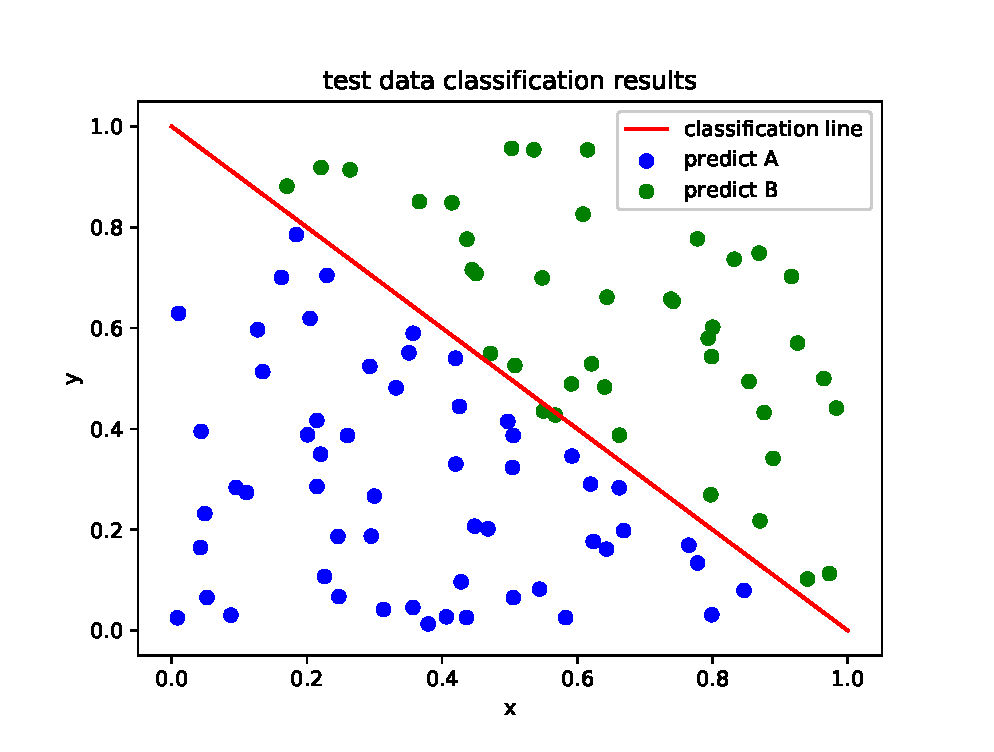
\includegraphics[scale=0.8]{sample_class.eps}
	\caption{简单二分类结果\label{fig:class_result}}
\end{figure}
\section{大展身手 --- 应用tensorflow实现对猫狗图集的分类}
\subsection{数据集说明}
本文所用的猫狗数据集来源于CSDN社区,共有训练图像25000张,其中猫12500张,狗12500张,其部分图像如图\ref{fig:simple_figure}。
\begin{figure}[h]
\centering
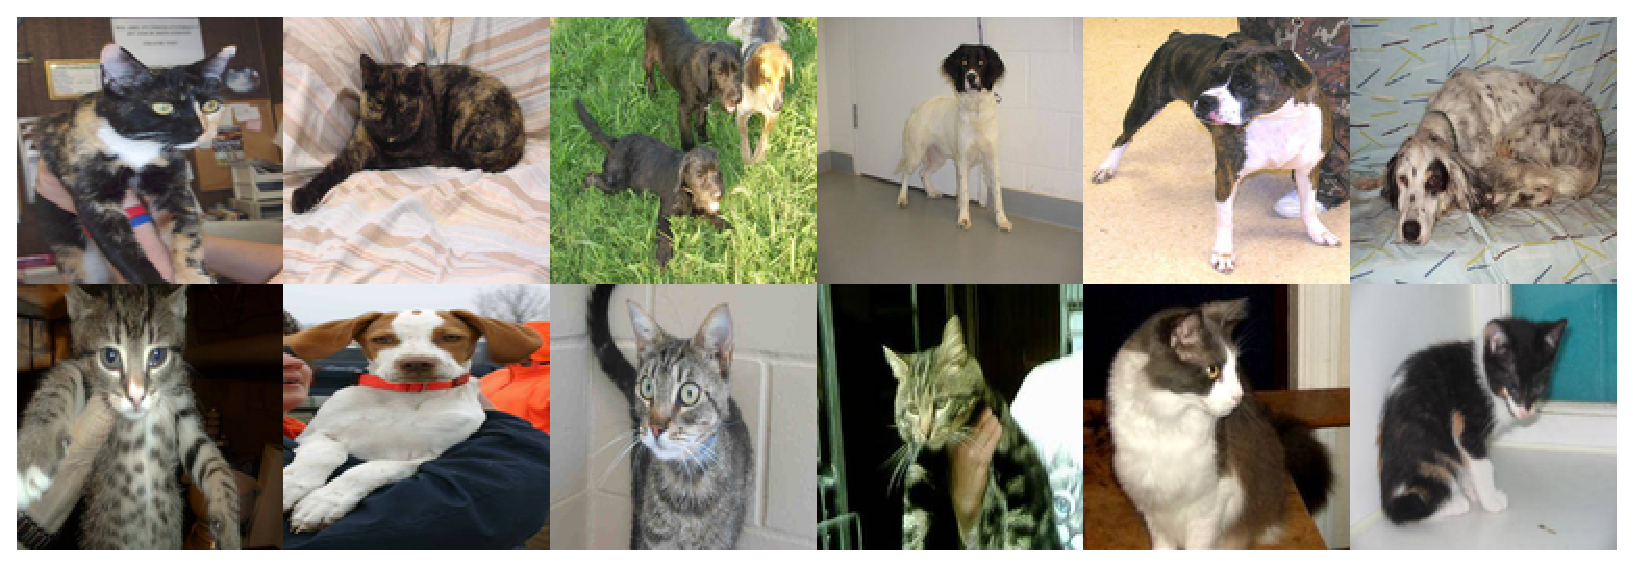
\includegraphics[scale=0.5]{final.eps}	
\caption{训练数据集数据样例\label{fig:simple_figure}}
\end{figure}
\subsection{卷积神经网络简介}
卷积神经网络(Convolutional Neural Network, CNN)是一种前馈神经网络,它的人工神经元可以响应一部分覆盖范围内的周围单元,对于大型图像处理有出色表现。卷积神经网络由一个或多个卷积层和顶端的全连通层(对应经典的神经网络)组成,同时也包括关联权重和池化层。这一结构使得卷积神经网络能够利用输入数据的二维结构。与其他深度学习结构相比,卷积神经网络在图像和语音识别方面能够给出更好的结果。这一模型也可以使用反向传播算法进行训练。相比较其他深度、前馈神经网络,卷积神经网络需要考量的参数更少,使之成为一种颇具吸引力的深度学习结构。常用的卷积神经网络架构,由输入层、卷积层1、池化层1、卷积层2、池化层2、全连接层1、全连接层2、softmax层、输出层这样几层组成。这种结构模型称为LeNet-5模型。
\subsection{tensorflow实现卷积神经网络结构}
本文考虑应用LeNet-5模型实现对猫狗图集的二分类。按上述模型的分层,逐层进行解释。
\begin{itemize}
	\item 输入层\\
	输入层是整个神经网络的输入,在处理图像的卷积网格中,输入层一般输入的为矩阵,在本文所考虑的图像为彩色的,考虑到通道,输入的为4维矩阵$208\times 208\times 3$。
	\item 卷积层1\\
	这一层输入的为原始的图像像素,按批次传入,本文每批次传入16张图像,卷积层过滤器的尺寸为3x3,深度为16,步长为1,共有16个偏置项。
	\inputpython{C:/Users/lsa/Desktop/deep_learning/cats_and_dogs/model.py}{7}{30}
	\item 池化层1\\
	这一层是卷积层1的输出,是一个$208\times 208\times16$本层采用的过滤器大小为$3\times3$,长和宽的步长均为2
	\inputpython{C:/Users/lsa/Desktop/deep_learning/cats_and_dogs/model.py}{32}{36}
	\item 卷积层2\\
	本层的输入矩阵大小为$104\times104\times 16$,使用的过滤器大小为$3\times 3$,深度为16。
	\inputpython{C:/Users/lsa/Desktop/deep_learning/cats_and_dogs/model.py}{37}{50}
	\item 池化层2\\
	本层的输入数据大小为$104\times 104\times 16$,采用过滤器大小为$3\times 3$,步长为1。
	\inputpython{C:/Users/lsa/Desktop/deep_learning/cats_and_dogs/model.py}{52}{55}
	\item 全连接层1\\
	本层输入矩阵大小为$104\times 104\times 16$。
	\inputpython{C:/Users/lsa/Desktop/deep_learning/cats_and_dogs/model.py}{57}{69}
	\item 全连接层2\\
	本层的输入节点个数为128,输出节点个数为128。
	\inputpython{C:/Users/lsa/Desktop/deep_learning/cats_and_dogs/model.py}{71}{82}
	\item softmax 层\\
	softmax层主要用于分类问题,运算得到术语不同种类的概率分布情况。
	\inputpython{C:/Users/lsa/Desktop/deep_learning/cats_and_dogs/model.py}{84}{96}
\end{itemize}
\subsection{tensorflow实现}
由于训练数据较多,共有25000张图片,不能直接将所有数据代入模型中进行训练,需要分批次代入,编写了一个批次获取函数,循环迭代,训练模型。训练完成后,从训练图片集中分别随机挑取20张猫和狗的图片,代入模型中得到预测结果,验证模型的正确性;然后尝试应用该模型取识别任意一张猫和狗的图片,应用网络爬虫技术从网上爬取了猫和狗的图片集,验证模型的通用性。tensorflow实现的流程图见图\ref{fig:process}。通过tensorflow工具包自带的可视化工具tensorboard,可以得到随着训练进行,正确率的变化趋势见图\ref{fig:train}。
\begin{figure}[ht]
	\centering
	\includegraphics[width=\linewidth]{train.png}
	\caption{随着训练中迭代进行模型识别准确率变化图\label{fig:train}}
\end{figure}
\subsubsection{训练模型的测试}
测试中从训练集中随机挑取了61张猫和狗的图片,代入模型,验证模型的准确性,结果见图\ref{fig:test_min}正确率为100\%。
\begin{figure}[hb]
	\centering
	\includegraphics[width=\linewidth]{test_min_result.png}
	\caption{模型测试结果\label{fig:test_min}}
\end{figure}
从结果上来看,该模型可很好的区分训练集中猫和狗。
\subsubsection{训练数据的获取---网络爬虫简单实现}
应用python工具包requests实现从百度图片中按猫或狗关键词抓取猫和狗的图片并保存到本地,收集好数据代入前模型中进行训练,结果见图\ref{fig:test_spyder},一共抓取了180张,猫狗各90张,正确率为57.76\%。
\begin{figure}
	\centering
	\includegraphics[width=\linewidth]{test_spyder.png}
	\caption{网络爬虫数据分类结果\label{fig:test_spyder}}
\end{figure}
从结果来看,通过训练集训练得到的模型不能较好识别网上获得的图片,主要原因是在网上这些图片中含有较多的干扰信息,如在一张图中既有猫又有狗,对分类造成影响。
\section*{感谢}
首先感谢胡海蔚同学提供的卷积神经网络模型工具,这给我的编程提供了很大帮助;其次感谢CSDN上额参考过的那些博主们,他们所提供的的解决问题的方法帮助我解决了许多环境配置或编写程序中的许多问题。
\newpage
\begin{thebibliography}{99}
	\songti %\zihao{-4} 
	\bibitem{1}郑泽宇,梁博文等,TensorFlow:实战Google深度学习框架,电子工业出版社,2018.2.
	\bibitem{2}刘大成,Python数据可视化之matplotlib实践,电子工业出版社,2018.9.
	\bibitem{3}张若愚,Python科学计算(第二版),清华大学出版社,2016.
	\bibitem{4}CSDN博客,https://blog.csdn.net/mbx8x9u/article/details/79124840
\end{thebibliography}

\begin{figure}
	\centering
	\includegraphics[width=0.8\linewidth]{process.png}
	\caption{猫狗图像集分类流程\label{fig:process}}
\end{figure}
\end{document}